\part{Graphs and trees}
\frame{\partpage}

\begin{frame}{Graphs}
	\begin{columns}
		\pause
		\begin{column}{0.3\textwidth}
			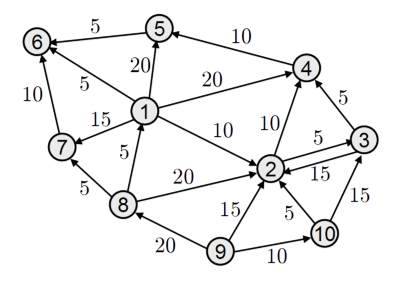
\includegraphics[width=\textwidth]{graph1}
			\par
			\vspace{2ex}
			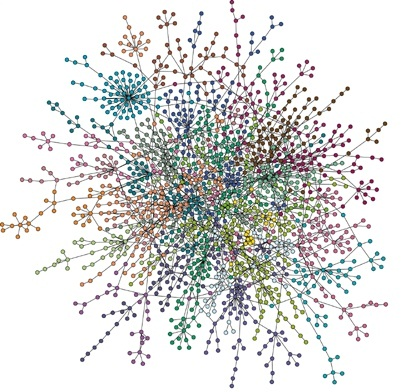
\includegraphics[width=\textwidth]{graph2}
		\end{column}
		\begin{column}{0.68\textwidth}
			\begin{itemize}
				\pause\item A \textbf{graph} is defined by:
					\begin{itemize}
						\pause\item A collection of \textbf{nodes} or \textbf{vertices} (points)
						\pause\item A collection of \textbf{edges} or \textbf{arcs} (lines or arrows between points)
					\end{itemize}
				\pause\item Often used to model \textbf{networks} (e.g.\ social networks, transport networks, game levels, automata, ...)
				\pause\item \textbf{Directed} graph: edges are arrows
				\pause\item \textbf{Undirected} graph: edges are lines
			\end{itemize}
		\end{column}
	\end{columns}
\end{frame}

\begin{frame}{Drawing graphs}
    \begin{itemize}
        \pause\item A graph does not necessarily specify the physical \textbf{positions} of its nodes
        \pause\item E.g.\ these are technically the same graph:
    \end{itemize}
    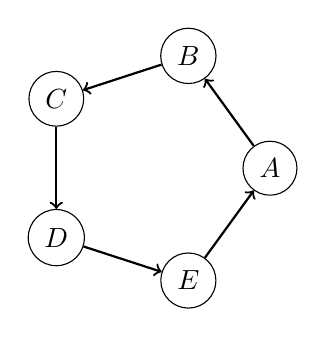
\begin{tikzpicture}
        \node[draw, circle] (a) at (0:1.5) {$A$};
        \node[draw, circle] (b) at (72:1.5) {$B$};
        \node[draw, circle] (c) at (144:1.5) {$C$};
        \node[draw, circle] (d) at (216:1.5) {$D$};
        \node[draw, circle] (e) at (288:1.5) {$E$};
        \draw[thick,->] (a) -- (b);
        \draw[thick,->] (b) -- (c);
        \draw[thick,->] (c) -- (d);
        \draw[thick,->] (d) -- (e);
        \draw[thick,->] (e) -- (a);
    \end{tikzpicture}
    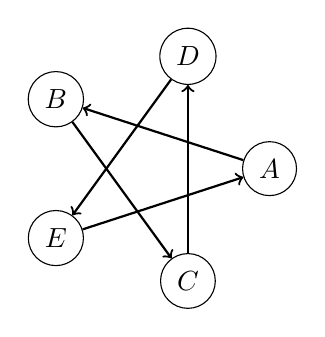
\begin{tikzpicture}
        \node[draw, circle] (a) at (0:1.5) {$A$};
        \node[draw, circle] (b) at (144:1.5) {$B$};
        \node[draw, circle] (c) at (288:1.5) {$C$};
        \node[draw, circle] (d) at (72:1.5) {$D$};
        \node[draw, circle] (e) at (216:1.5) {$E$};
        \draw[thick,->] (a) -- (b);
        \draw[thick,->] (b) -- (c);
        \draw[thick,->] (c) -- (d);
        \draw[thick,->] (d) -- (e);
        \draw[thick,->] (e) -- (a);
    \end{tikzpicture}
    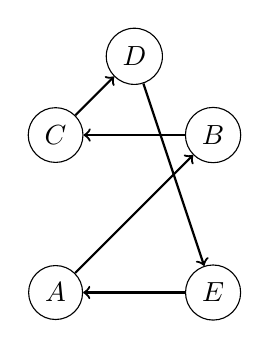
\begin{tikzpicture}
        \node[draw, circle] (a) at (0,0) {$A$};
        \node[draw, circle] (b) at (2,2) {$B$};
        \node[draw, circle] (c) at (0,2) {$C$};
        \node[draw, circle] (d) at (1,3) {$D$};
        \node[draw, circle] (e) at (2,0) {$E$};
        \draw[thick,->] (a) -- (b);
        \draw[thick,->] (b) -- (c);
        \draw[thick,->] (c) -- (d);
        \draw[thick,->] (d) -- (e);
        \draw[thick,->] (e) -- (a);
    \end{tikzpicture}
\end{frame}

\begin{frame}{Trees}
	\begin{columns}
		\pause
		\begin{column}{0.3\textwidth}
			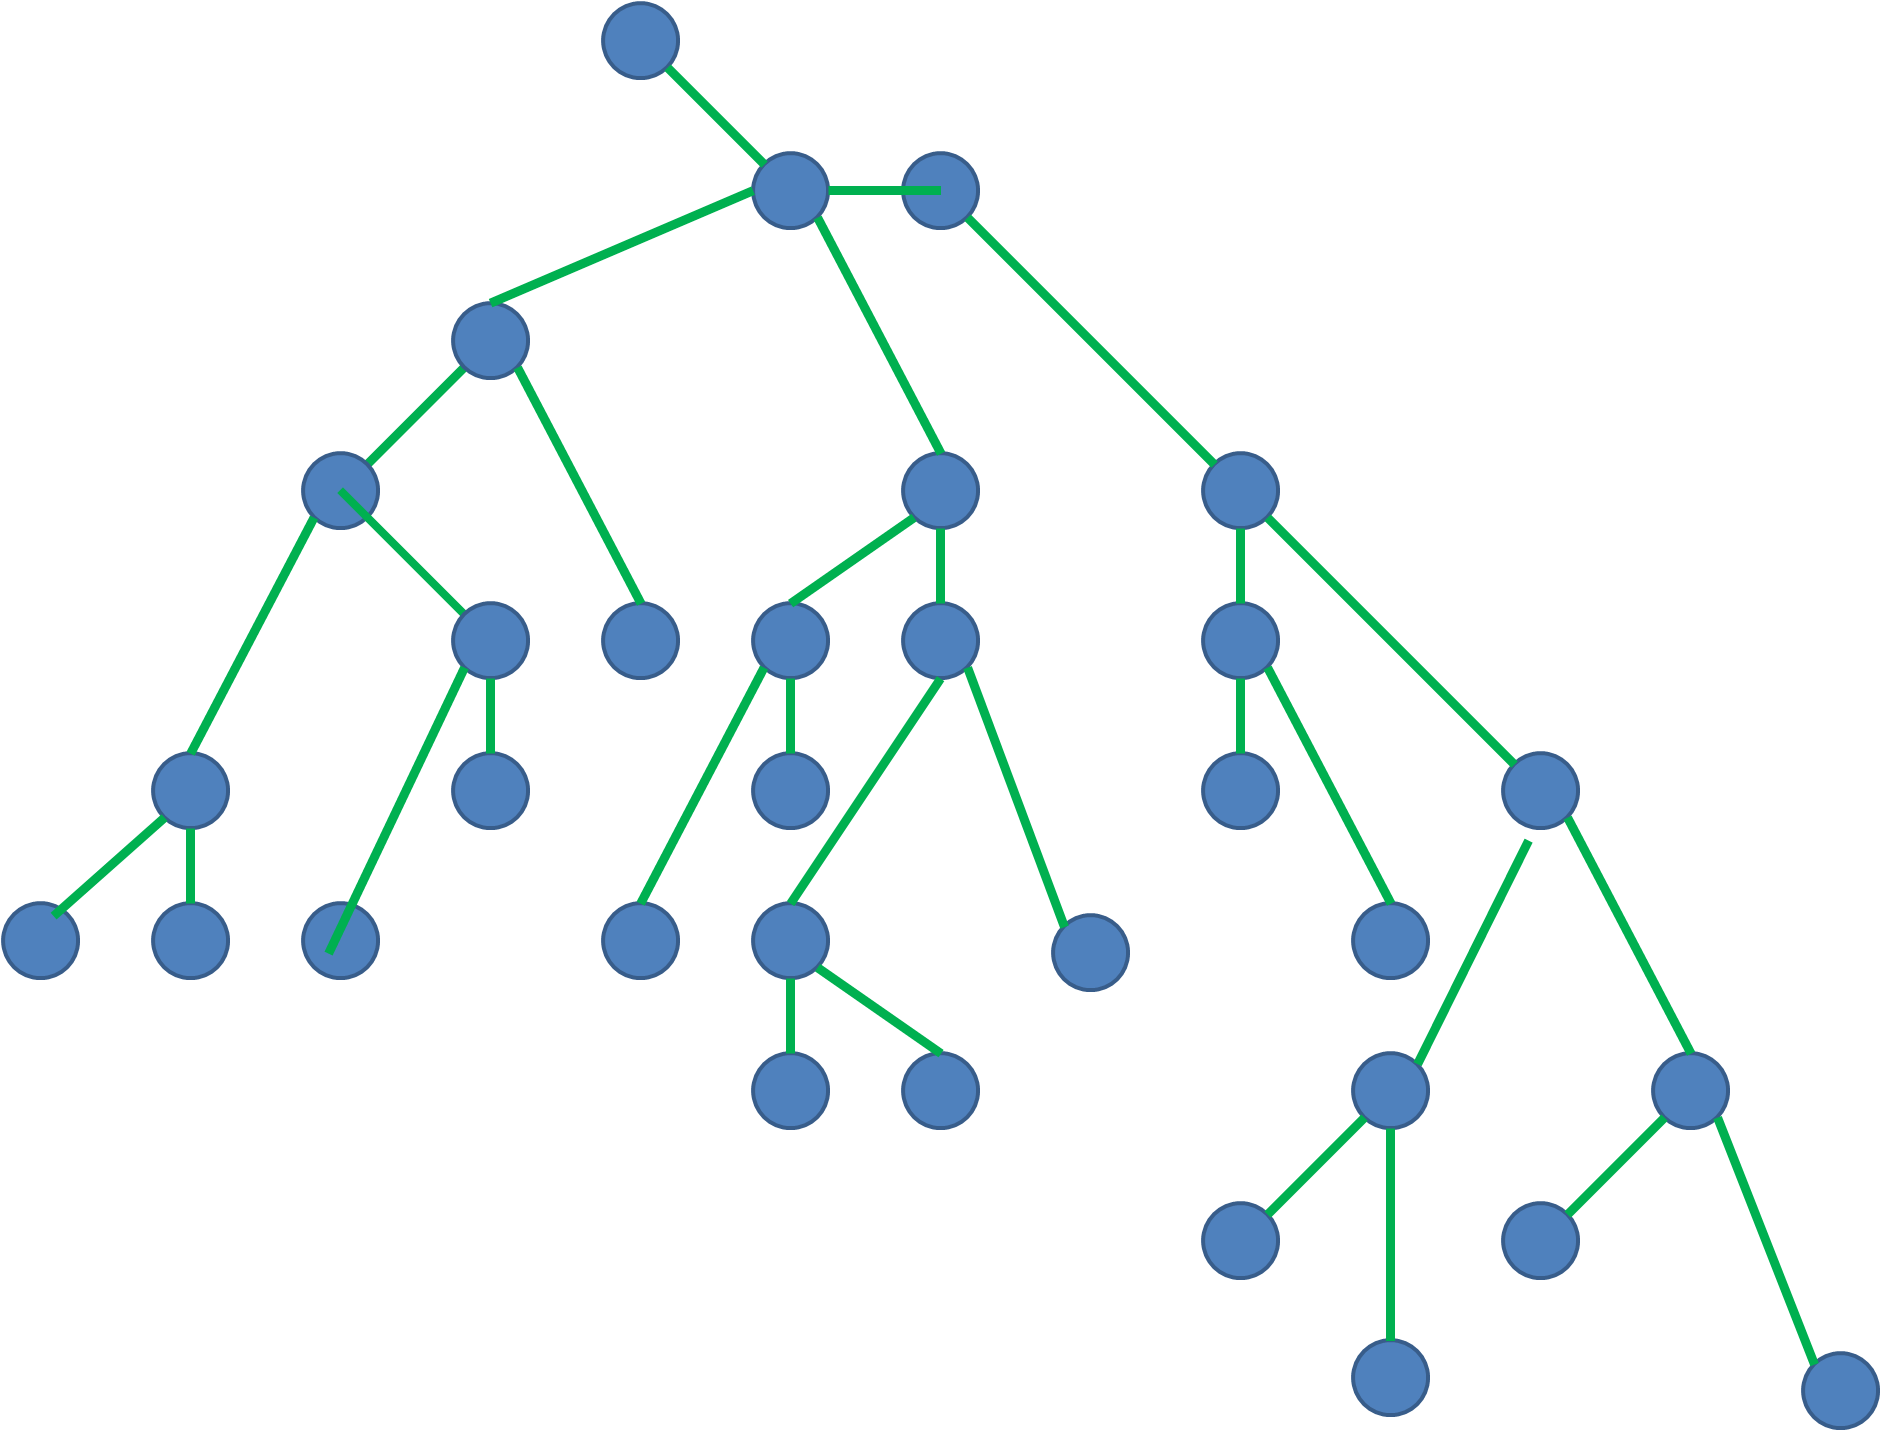
\includegraphics[width=\textwidth]{tree2}
			\par
			\vspace{2ex}
			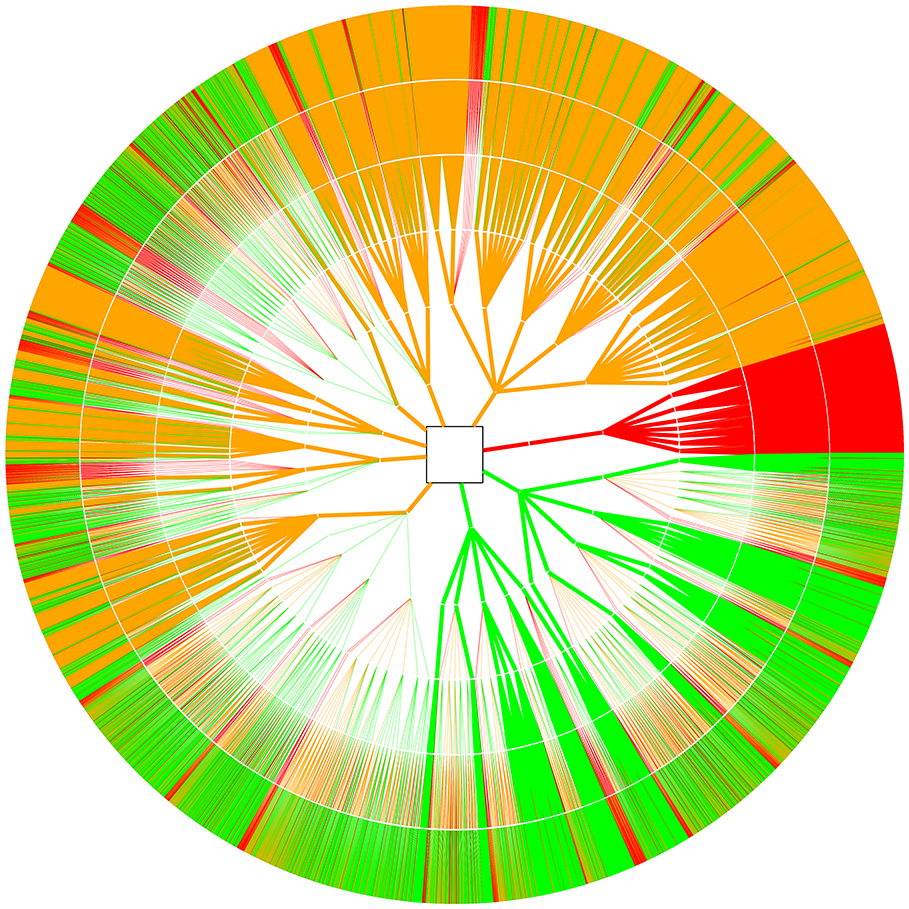
\includegraphics[width=\textwidth]{tree}
		\end{column}
		\begin{column}{0.68\textwidth}
			\begin{itemize}
				\pause\item A \textbf{tree} is a special type of directed graph where:
					\begin{itemize}
						\pause\item One node (the \textbf{root}) has no incoming edges
						\pause\item All other nodes have exactly 1 incoming edge
					\end{itemize}
				\pause\item Edges go from \textbf{parent} to \textbf{child}
					\begin{itemize}
						\pause\item All nodes except the root have exactly one parent
						\pause\item Nodes can have 0, 1 or many children
					\end{itemize}
				\pause\item Used to model \textbf{hierarchies} (e.g.\ file systems, object inheritance, scene graphs, state-action trees, behaviour trees, ...)
			\end{itemize}
		\end{column}
	\end{columns}
\end{frame}
